\section{Introduction}

Cilia are microtubule-based hair-like projections of cells; in humans, they are found on nearly every cell of the body. Disorders known as ciliopathies, where cilia function is disrupted, can result in a wide spectrum of diseases. In primary ciliary dyskinesia (PCD), airway cilia that normally beat in synchrony to mediate mucus clearance can exhibit dyskinetic motion or become immotile, resulting in severe sinopulmonary disease\cite{o2007diagnosing}. Cilia defects have been associated with increased respiratory complications and poor post-surgical outcomes \cite{nakhleh2012high}. The characterization of ciliary motion abnormalities and specifics of the ciliary motion properties itself plays a critical role in the identification of specific ciliopathy and the determination of prophylactic respiratory therapies that could improve long-term outcomes in patients. Therefore, accurate identification of specific ciliary motion patterns is clinically compelling.

An objective, computational method for quantitative assessment of ciliary motion was proposed in by Quinn in 2015 \cite{quinn2015automated}. In his work, ciliary motion was considered as an instance of dynamic texture \cite{saisan2001dynamic}. Dynamic textures are modeled as rhythmic motions of particles subjected to stochastic noise \cite{chen2013automatic}. Examples of dynamic textures include familiar motion patterns such as flickering flames, rippling water, and grass in the wind, each with a small amount of stochastic behavior altering an otherwise regular visual pattern. Ciliary motion is well described as a dynamic texture. This representation proved robust for normal/abnormal binary ciliary motion classification, achieving an accuracy of over 90\% relative to expert ground-truth labeling.

While this study was instrumental in establishing the efficacy of dynamic textures as quantitative representations for ciliary motion, it had some critical limitations, such as the use of autoregressive (AR) models \cite{hyndman2007higher} to model ciliary motion. While AR models are the preferred representation of dynamic textures, their primary use is in distinguishing between \textit{different} types of dynamic textures, rather than between different instances of the \textit{same} dynamic texture. Furthermore, the strong parametric assumptions imposed by the AR model on the underlying structure of the data -- multivariate Gaussian generating distributions that live on a linear manifold -- severely restrict the representative power of AR models, truncating their sensitivity to minor but important variations in motion dynamics and rendering them incapable of capturing complex, nonlinear interactions.

Also, despite the considerable effort in automating much of the quantitative motion analysis, the authors still ultimately relied on expert clinician collaborators to manually select and extract regions of interest (ROI) from the raw video data to focus the analysis of the computational pipeline. These ROIs potentially introduce the same subjective bias of individual preference and training into the resulting data.

Here, we examine the application of deep learning, specifically \textit{convolutional neural networks} (CNNs) to perform binary ciliary motion classification. CNNs do not impose strong parametric assumptions on the underlying data and instead capture complex dynamics and interdependencies through a series of convolutional filters. Furthermore, CNNs do not require manual ROI to be selected and can automatically learn which areas of the videos are relevant to building feature maps.

3D CNNs provide a more scalable solution to ciliary motion classification while still incorporating information about the temporal structure inherent to the video data of cilia biopsies.

\section{Methods}

The objective of this experiment was to establish a baseline accuracy with a deep learning approach to cilia classification. To take advantage of the temporal dimension of video, an artificial neural network with 3D convolution filters was implemented to classify abnormality in cilia motion. Similar computer vision techniques were used to preprocess the raw video data from previous studies  \cite{quinn2011novel}; specifically, the derivatives of optical flow were computed from the cilia videos and differential flow invariants (rotation) were extracted and fed into the 3D CNN in batches of frames.

The dataset comprised of grayscale videos from nasal brush biopsies on 149 patients and examined by a blinded panel of clinicians. These videos were recorded at 200 frames per second for several seconds, and taken at $640 \times 480$ resolution (Fig.~\ref{fig:cilia}). The panel of experts assigned labels to each patient to indicate the degree of abnormal cilia motion in the videos, where 1 constituted completely normal motion, 4 constituted highly abnormal motion, and 2 and 3 expressed gradations of abnormality. 

\begin{figure}[htp]
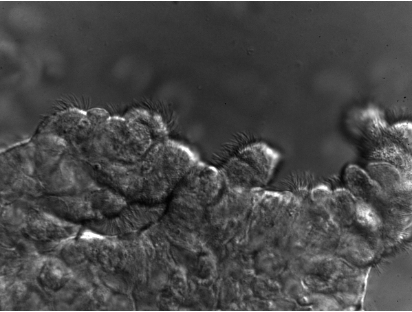
\includegraphics[scale=0.78]{grey_1011-5_heathly}
\caption{Example frame of a ciliary video labeled as normal; the regions containing cilia are evident along the cell boundaries.}
\label{fig:cilia}
\end{figure}

Multiple videos per patient were collected, and each video was given the label of its patient. Some video samples were removed due to extraneous camera movement, poor lighting, or other recording artifacts. Videos of patients with labels of 2 and 3 were removed from the training set to leave more canonical examples of normal and abnormal motion for the network to learn better representations. Out of the total 325 videos, 266 (81.85\%) canonical videos were used to train the network. From this subset, 127 videos (47.77\%) were labeled as examples of abnormal cilia motion, while the rest of the videos were labeled as examples of normal motion.
 
Optical flow is used in computer vision to predict the probable motion of pixels between consecutive frames and represents the movement of a pixel as a displacement vector field. Taking linear combinations of the derivatives of optical flow yields differential image invariants, also known as the measures: rotation, divergence, and deformation. These quantities are orientation-invariant, allowing ciliary motion to be analyzed irrespective to camera orientation, lighting differences, and even the direction the cilia beats~\cite{quinn2015automated}. The computed curl (rotation) of ciliary motion was used for training because it was the only scalar valued component (divergence and deformation being vector quantities). 
 
The videos were standardized to the absolute maximum value in order to preserve the most information when converting from floating point to 16 bit integer values. Some videos had extremely high maximum values so scalars for each video were individually computed to prevent pixel overflow while maximizing the range of the integer data type. Each video had 250 frames, which were each reduced from $640 \times 480$ to $80 \times 60$ pixels and split into blocks of 10, effectively producing 25 arrays of $80 \times 60 \times 10$ inputs per video. These blocks of arrays were fed in batches of 10 per iteration into a 3D CNN that was implemented in TensorFlow and trained on a p2 instance from Amazon Web Services (AWS). 

\begin{figure*}
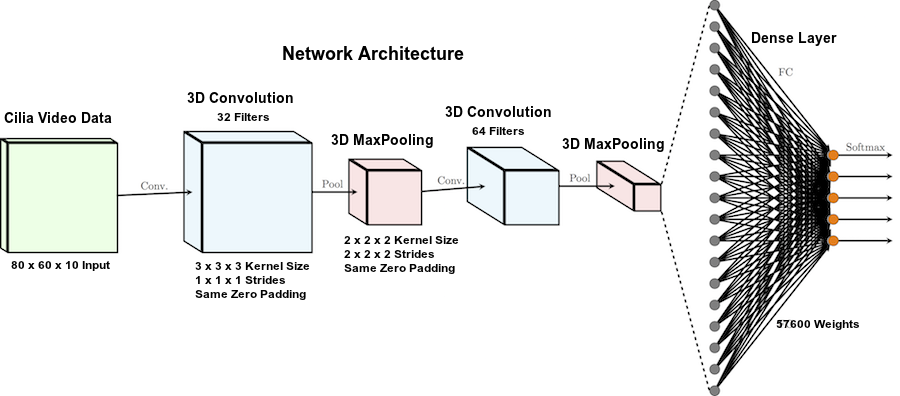
\includegraphics[scale=1.2]{arch}
\caption{Overview of the 3D CNN architecture as implemented in TensorFlow.}
\label{fig:cnn}
\end{figure*}
%\setlength{\textfloatsep}{5pt}

\section{Results}

The 3D CNN architecture had 2 stacked layers, each composed of a 3D convolution layer, a 3D max pooling layer, and a layer with Rectified-Linear Unit \cite{nair2010rectified} activation functions. These two layers fed into a fully connected dense layer that outputted to a binary softmax classifier. Most CNN ``best'' practices \cite{goodfellow_bengio_courville_2016} were adapted for three dimensions. The first layer had 32 3D convolutional filters and the second layer had 64 filters. The kernel size of each filter was $3 \times 3 \times 3$ with zero padding used and dropout \cite{srivastava2014dropout} added for regularization. The fully connected layer had 57600 weights ($80 * 60 * 10 = 48,000$ plus 9,600 extra weights from the zero padding). A visualization of the network architecture is shown in Fig.~\ref{fig:cnn}.

An adaptive learning rate was used with the ADAM~\cite{kingma2014adam} optimizer. A low batch size of 10 was selected to accommodate the memory capacities of our hardware resources. After 10 iterations, the model converged to a local minimum. We tested classification accuracy with a 66-33\% train-test split. 

The average performance of the 3D CNN on the test set was around 75\%, which is below the 90\% benchmark accuracy from~\cite{quinn2015automated}; see Fig.~\ref{fig:iterations}. Using larger batch sizes and pixel dimensions slightly improved performance but at the cost making the model much more computationally expensive and exhausted memory capabilities of our machine. Trading dimension size of each frame for a larger block size had little difference in terms of accuracy but also greatly increased computational requirements.  

\begin{figure}
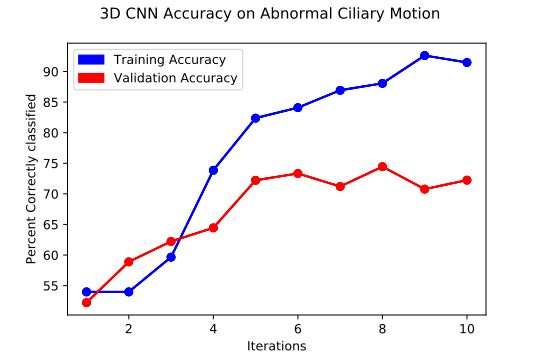
\includegraphics[scale=0.5]{CNN_graph}
\caption{Training and testing accuracy of the 3D CNN as a function of network epochs.}
\label{fig:iterations}
%\setlength{\belowcaptionskip}{-10pt}

\end{figure}


\section{Discussion}

Clearly, the model is severely overfitting the dataset. Several regularization techniques could be implemented to combat this: transfer learning from pre-trained networks, data augmentation, and batch normalization. However, each pose their own difficulties. For transfer learning, most pre-trained network weights are designed for image input rather than video data \cite{pan2010survey}. Data augmentation is feasible but must be done congruently within batches which would require more processing power for videos than images when done in memory. Also, the underlying structure of the processed data might not allow for some of the same transformations as the raw grayscale videos. Batch Normalization \cite{ioffe2015batch} would be rather straightforward to implement but seems unlikely to improve current classification accuracy to the state of the art benchmark. From already experimenting with the dropout regularization parameter, the learning capacity of the 3D CNN seems too complex for the down-sampled data. We believe a better solution would be to provide the model with more labeled training examples and enough computing resources to allow for larger input dimensions. 
 
One limitation of the data was each video had the label at a patient level instead of each individual video, which might not contain any abnormal motion at all despite the patient being labeled abnormal or vise versa. Also, a training example might contain multiple cells with some showing normal motion and others having abnormal motion within the same video. We attempted to mitigate the effect of these misleading examples by following Bengio's \cite{bengio2009curriculum} idea of curriculum learning, opting to train only on patients labeled 1 and 4 (trading quantity of training examples for more canonical videos).

Another limitation was the drastic reduction in pixel dimensions of the cilia data. The processed videos had to be reduced to $\frac{1}{8}$ their original size to avoid into memory limits. This downsampling greatly diminished the network's capacity to extract relevant features and discriminate between normal and abnormal ciliary motion. With more computing resources and a more precisely labeled dataset, we expect an increase in classification accuracy with 3D CNN. With additional preprocessing, the deformation vector data could also be incorporated in addition to the rotation data to provide even more contextual information for network to learn better representations about the dynamics of ciliary motion.

\section{Conclusion}

Although deep learning methods usually requires an abundant amount of labeled training data, one possible way to circumvent this issue would be to train another CNN to automatically generate a heat-map of candidate areas of the video where cilia are likely to be present, similar to the deep learning pipeline \cite{wang2016deep} that won the Camelyon 17 challenge for breast cancer classification. Then, feed this into another classifier such as a Gradient Boosted Decision Tree or even another CNN to predict the probability of abnormality on that region of cilia.
 
Other approaches that could leverage deep learning for cilia classification are Recurrent Neural Networks (RNNs) such as a Long-Short Term Memory (LSTM) network, which inherently incorporates the dimension of time into account to build feature maps. It is even possible to stack CNNs on top of RNNs to leverage aspects of both network architecture types. Other researchers \cite{sonderby2015convolutional} have already applied a similar approach with promising results on localization of protein structures. Another interesting area of deep learning that holds promise to solve the broader issues of cilia segmentation and identification of different ciliary motion phenotypes include the attention-seeking mechanisms to segment out cilia and General Adversarial Networks to generate a canonical phenotype of a specific ciliary motion.

\section{Acknowledges}

The authors would like to acknowledge the University of Pittsburgh and Children's Hospital of the University of Pittsburgh Medical Center for initial acquisition of video microscopy data. In particular, we would like to acknowledge and thank Dr. Chakra Chennubhotla, Dr. Maliha Zahid, and Dr. Cecilia Lo.


%\end{document}  % This is where a 'short' article might terminate
